%\chapter*{Введение}
%\addcontentsline{toc}{chapter}{Введение}

\newpage
\begin{center}
\textbf{ГЛАВА 2}\\
\textbf{КОЛЛЕКТИВНЫЕ СПЕКТРЫ В КОНДЕНСИРОВАННЫХ СИСТЕМАХ}
\end{center}
\refstepcounter{chapter}


% \section*{}
\addcontentsline{toc}{chapter}{ГЛАВА 1. Коллективные спектры в конденсированных системах}
\section{Расчет спектров в МД}

%Значительное число ключевых свойств конденсированного вещества определяется спектрами элементарных возбуждений и, в частности, коллективных колебаний. Однако поведение и описание коллективных мод в неупорядоченных средах (например, жидкостях и стеклах) остается сложной областью современной науки о конденсированных средах. В последнее время теоретически предсказывалось и наблюдалось в молекулярно-динамическом моделировании антикроссинга между продольными и поперечными модами, но это фундаментальное явление никогда не наблюдалось экспериментально. 

Коллективные возбуждения являются одной из ключевых концепций современной
физики конденсированного состояния ~\cite{dove_1993, HansenMacDonald, landau.statphys}. Это обусловлено тем,
что знание коллективных возбуждений в конденсированной системе позволяет
понять многие свойства системы, такие как: термодинамические, упругие,
структурные и т.д. Коллективные возбуждения в случае кристаллических систем
являются наиболее изученными. Главным образом благодаря наличию
трансляционной симметрии и малости отклонений частиц кристаллической решетки
от положений равновесия. Трансляционная симметрия позволяет рассматривать
коллективные возбуждения в кристалле как плоские волны, а малость
отклонений позволяет рассматривать как гармонические невзаимодействующие
колебания. В физике твердого данные колебания принято отождествлять
с квазичастицами - фононами. При высоких температурах отклонения
частиц становятся большими и фононы уже нельзя рассматривать как невзаимодействующие.


В случае жидкостей так же можно говорить о коллективных возбуждениях,
однако они имеют более сложную структуру и хуже изучены. Однако
существует теоретический подход к оценке дисперсионных зависимостей в жидкостях,
известный, как QCA (quasi-crystalline approximation) ~\cite{Khrapak:2018aa}. Во многих
случаях описание на основе QCA справедливо и согласуется с дисперсионными
кривыми, полученными экспериментально, для различных простых жидкостей,
по крайней мере.


В контексте физики плазмы первоначально был предложен аналог QCA -- подход QLCA (quasi-localized charge approximation) ~\cite{doi:10.1063/1.873814}, который использовался для расчета дисперсии  коллективных мод в  сильно коррелированной жидкой фазе.
%случае различных кулоновских систем, бинарных ионых смесей, электронных бислоев, однокомпонентной системы Юкавы в

Метод был создан для сильно связанных систем, где традиционная аппроксимация рандомной фазы RPA (random-phase approximation) или иерархия ББГКИ не была бы оправдана. Теория QLCA позволила предсказать дисперсию плазменных и сдвиговых мод не только в упомянутых выше системах, но и в намагниченной однокомпонентной плазме и в электронных сверхрешетках.

Подход QCA связывает динамические и структурные характеристики системы,
то есть позволяет рассчитать дисперсионные соотношения для коллективных
возбуждений в жидкости, на основе потенциальной энергии парного взаимодействия
и парной-корреляционной функции $g(r)$.
Однако обратная процедура плохо изучена, и теория восстановления парных
корреляций с использованием потенциала взаимодействия и динамических свойств
хорошо развита только для кристаллов \cite{10.1039/C7SM02429K, Khrapak:Practicalth, Yurchenko2016IM}.

Для анализа различных подходов к построению спектров элементарных возбуждений было проведено моделирование на основе методов молекулярной динамики (МД) с использованием NVT ансамбля.
Рассматривался метод построения на основе простых жидкостей с потенциалами Леннарда-Джонса и Юкавы:

\begin{equation}
\varphi_{LJ} = 4 \varepsilon \Big[\Big(\frac{\lambda}{r} \Big)^{12} - \Big(\frac{\lambda}{r} \Big)^6\Big],
\end{equation}

\begin{equation}
\varphi_{Y} = \varepsilon \frac{\lambda}{r} \Big(-\frac{r}{\lambda} \Big),
\label{Yukawa}
\end{equation}


где $\varepsilon$ и $\lambda$ – магнитуда и характерная длина взаимодействия соответственно.

В случае систем с потенциалом Леннарда-Джонса система состояла из $N = 10^4$ частиц с радиусом отсечки $r_c = 7.5 n^{-1/D}$, где $n = N/V$ - плотность, а $D$ - размерность системы. Моделирования проводились с временным шагом $\Delta t = 5 \times 10^{-3} \sqrt{T_0 m \sigma^2/(T\epsilon)}$.



Для рассмотренной системы на основе данных, полученных в результате моделирования, были рассчитаны плотности потока скоростей на основе фурье-преобразования \cite{Khrapak:2018aa}:\\
\begin{equation}
C_{L, T}(q, \omega) = \int dt e^{i\omega t} Re \langle \mathbf{j}_{L,T} (\mathbf{q}, t) \mathbf{j}_{L,T} (-\mathbf{q}, 0)\rangle,
\label{VelCurrent}
\end{equation}

\noindent
где $\mathbf{j}_{L,T} (\mathbf{q}, t) = N^{-1}\sum_s \mathbf{v}_s(t)exp(i \mathbf{qr}_s(t))$ - плотность потока скоростей; $\mathbf{v}_s(t) = \dot{\mathbf{r}}_s(t)$ - это скорость s-ой частицы; суммирование проводилось по всем $N$ частицам системы. $\mathbf{j}_L = \mathbf{q}(\mathbf{j\cdot q})/q^2$ и $\mathbf{j}_T = \mathbf{j} e_{\bot}$ - продольные
и поперечные компоненты потока, $e_{\bot}$ - единичный вектор, нормальный к $\mathbf{q}$; скобки $\langle \cdots \rangle$ обозначают усреднение по каноническому ансамблю.


В связи с изотропностью простых жидкостей, спектры потоков частиц зависят только от частоты $\omega $ и волнового числа $q = |\mathbf{q}|$. Пользуясь этим свойством, значение $C_{L, T}(\mathbf{q}, \omega)$ 
усреднялось по всем направлениям волнового вектора для подавления шума, вызванного ограниченностью набора частиц и времени моделирования:


\begin{equation}
C_{L, T}(q, \omega) = \frac{1}{N_q}\sum_{q = |\mathbf{q}|} C_{L, T}(\mathbf{q}, \omega),
\label{VelCurrentMean}
\end{equation}

\noindent
где $N_q$ -- количество направлений, используемых для усреднения.

Данный подход применим при условии $\mathbf{q} \lesssim 2\pi /L$, где
$L$ -- характерный размер области моделирования. Предполагается, что спектры потоков частиц имеют следующий вид:

\begin{equation}
Re \langle \mathbf{j}_{L,T} (\mathbf{q}, t) \mathbf{j}_{L,T} (-\mathbf{q}, 0)\rangle \propto e^{-\Gamma _{L, T}(q)|t| }cos(\omega_{L,T}(q)t),
\label{Doe}
\end{equation}

\noindent
где $\omega_{L, T}$ и $\Gamma_{L, T}$ - частота и коэффициент затухания соответственно для продольных и поперечных колебаний. Таким образом, получается следующее выражение для спектров потоков частиц (DHO модель):

\begin{equation}
C_{L, T}(q, \omega) \propto \frac{\Gamma_{L, T}(q)}{(\omega - \omega_{L, T}(q))^2 + \Gamma^2_{L, T}(q)} + \frac{\Gamma_{L, T}(q)}{(\omega + \omega_{L, T}(q))^2 + \Gamma^2_{L, T}(q)}.
\label{DHO}
\end{equation}

Частоты и коэффициенты затухания (\ref{VelCurrentMean}) можно так же получить как раздельной аппроксимацией (\ref{DHO}) продольных и поперечных колебаний, так и совместной аппроксимацией (модель 2DHO), при котором полный спектр
$C(q, \omega) = C_L (q, \omega)+ (D -1) C_T(q, \omega)$ получается в виде суммы двух аппроксимаций высокочастотных и низкочастотных колебаний:

\begin{equation}
C(q, \omega) \propto \frac{\Gamma_{L}}{(\omega - \omega_{L})^2 + \Gamma^2_{L}} + \frac{\Gamma_{L}}{(\omega + \omega_{L})^2 + \Gamma^2_{L}} + \frac{(D - 1) \Gamma_{T}}{(\omega - \omega_{T})^2 + \Gamma^2_{T}} + \frac{(D - 1)\Gamma_{T}}{(\omega + \omega_{T})^2 + \Gamma^2_{T}},
\label{2DHO}
\end{equation}

\noindent
где $D$ -- это размерность системы.

\begin{figure}[htbp!]
\begin{center}
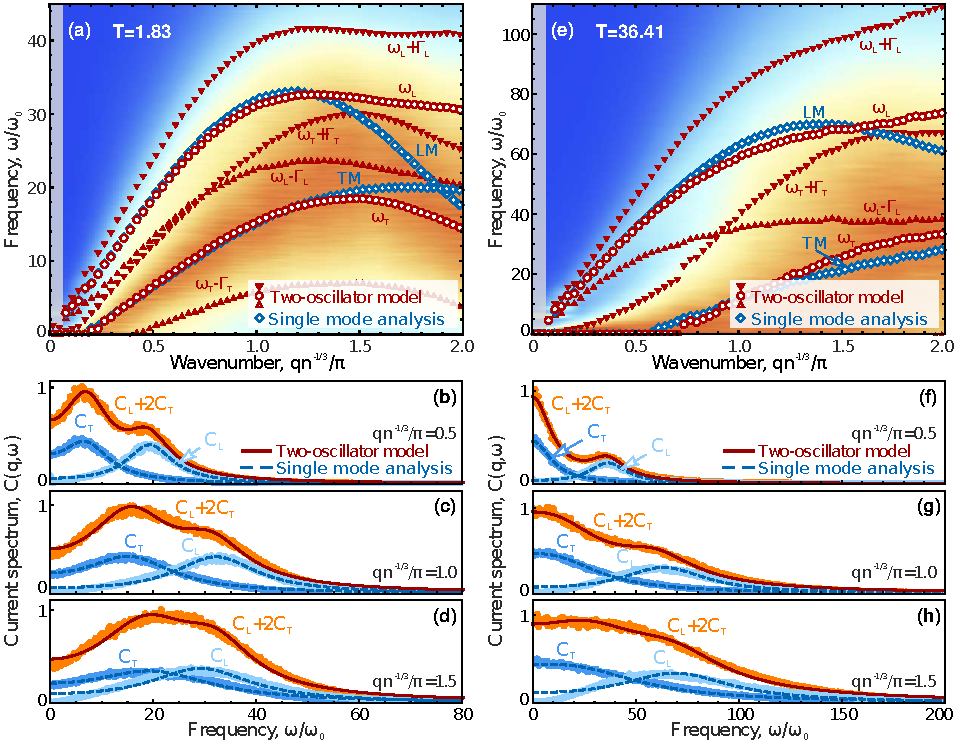
\includegraphics[width=0.7\textwidth]{Ris/CFS-Figure1.pdf}
\caption{Амплитуды и спектры возбуждений для трехмерной жидкости с потенциалом Леннарда-Джонса. }
\label{VelCurrent}
\end{center}
\end{figure}

Оба метода дают зависимости с разбросом значений частот $\omega_{L,T}(q)$ и коэффициентов взатухания $\Gamma_{L, T} (q)$. На рис. \ref{VelCurrent} можно увидеть результаты для Леннарда-Джонса при низких (a) - (d) и высоких (e) - (h)
температурах (T = 1.83 и 36.41 соответственно).




% (a) Спектр потока частиц $C(q, \omega)$ изображен в цветовом формате при $T = 1.83$ и $n = 1$, дисперсионные соотношения $\omega_{L, T}(q)$, полученные раздельной аппроксимацией, обозначены синими ромбами, соответствующими продольным и поперечным модам, а те, что получены совместной аппроксимацией, обозначены красными кругами. Треугольники
% соответствуют $\omega_{L, T} \pm \Gamma_{L, T}$. Зоны, обозначенные серым, соответствуют областям $qn^{-1/3} < 2\pi / L$. Панели (b) - (d) демонстрируют участки спектров потоков частиц при различных $qn^{-1/3}
% / \pi = 0.5, 1.0$ и $1.5$, полученных из моделирования (обозначены символами), и результаты аппроксимирования моделью 2DHO (5) и DHO (4) (показаны сплошной
% красной и пунктирными синими линиями соответственно). На панелях (e) - (h) аналогичные результаты, но полученные при T = 36.41 и n = 1.




На рис. \ref{VelCurrent}(а) представлены результаты $C (q, \omega)$ в цветовом формате. Синие ромбы соответствуют
дисперсионным соотношениям $\omega_{L, T} (q)$, рассчитанным путем раздельной аппроксимации продольной и поперечной мод. Результаты, полученные с помощью совместной аппроксимации,
показаны красными кругами для $\omega_{L, T} (q)$ и треугольниками для
$\omega_{L, T} (q) \pm \Gamma_{L, T}$. Результаты, полученные с помощью модели DHO, не изображены, поскольку они совпадают с теми, что уже показаны на рисунке. Профили $C (q, \omega)$, а также их продольные и поперечные составляющие $C_{L, T} (q, \omega)$ для различных значений волнового числа изображены на рис. \ref{VelCurrent}(b) - (d) символами, в то время как сплошные линии соответствуют результатам аппроксимации по формулам (\ref{DHO}) и (\ref{2DHO}).


Следует отметить, что оба подхода дают близкие
результаты, если полный спектр $C (q, \omega)$ имеет два хорошо выраженных максимума (на более низких и более высоких частотах, которые
обычно соответствуют продольным и поперечным модам), что обычно выполняется в первой псевдозоне Бриллюэна. Отклонение между дисперсионными соотношениями, полученными различными методами, растет с ростом температуры, как видно на рис. \ref{VelCurrent}(а) и \ref{VelCurrent}(е). Видно, что результаты,
полученные методами молекулярной динамики, хорошо согласуются с теоретическими подходами (\ref{DHO}) и (\ref{2DHO}).


При больших температурах и коротких
длинах волн, как показано на рис. \ref{VelCurrent}(h), результаты сильно искажаются, что связано с
изменением формы спектров на длинноволновом пределе. Если попереречные и продольные волны пересекаются, то модель DHO становится неприменимой (при $qn^{-1/3}/ \pi \simeq 1.9$). Смешивание мод и эффективное взаимодействие между ними сопровождается сильным перераспределением спектров и гибридизацией \cite{101103, 112101}.






\section{Анализ спектров в комплексной (пылевой) плазме}



%Теория, моделирование и эксперименты наглядно демонстрируют наличие антикроссинга мод, которое сопровождается гибридизацией и сильным перераспределением спектров возбуждения.


Для анализа скрещивания мод в сильно связанных жидкостях с потенциалом Юкавы было проведено моделирование МД для квазидвумерной жидкости при  $\varepsilon = e^2 Z^2 /4\pi \varepsilon_0 \lambda_D = 874 ~\text{эВ}$, где $Z = 1.25 \times 10^4$ - зарядовое число, $\lambda_D  = 260~ \text{нм}$ - длина экранировки Дебая. 

Система состояла из $N = 10^4$ частиц с массами, равными $m = 6.1 \times 10^{-10}~ \text{гр}$, помещенными в кубическую область с периодическими граничными условиями со сторонами $L = 30.5~ \text{м}$. Частицы находились в параболической потенциальной яме $U(z)  = 0.5 m \Omega_z^2 z^2$, где $\Omega_z^2 = 25 ~\text{Гц}$ - частота поперечных колебаний частиц  в длинноволновом пределе. 



Радиус отсечки был взят равным $r_c = 2.29~ \text{мм}$, что примерно соответствовало 7.5 межчастичных расстояний. Моделирование проводилось в термостате Ланжевена с $T = 18~ \text{эВ}$, скоростью затухания $\nu = 1.8 ~\text{с}^{-1}$ и шагом по времени $\Delta t = 38~ \text{нс}$. На начальном этапе была задана квадратная решетка в плоскости $z = 0$ с плотностью $\rho = 1/V_0 = N/L^2 = 10.75~ \text{мм}^{-2}$ при температуре $T = 26.9~ \text{эВ}$ (которая соответствует распределению Максвелла). Первые $10^{6}$ шагов система находилась в состоянии равновесия, затем следующие $10^6$ шагов были использованы для анализа спектров флуктуаций.




На рис. \ref{PlasmaSp} изображены спектры элементарных возбуждений для квазидвумерных жидкостей с потенциалом Юкавы. 

\begin{figure}[htbp]
    \begin{center}
    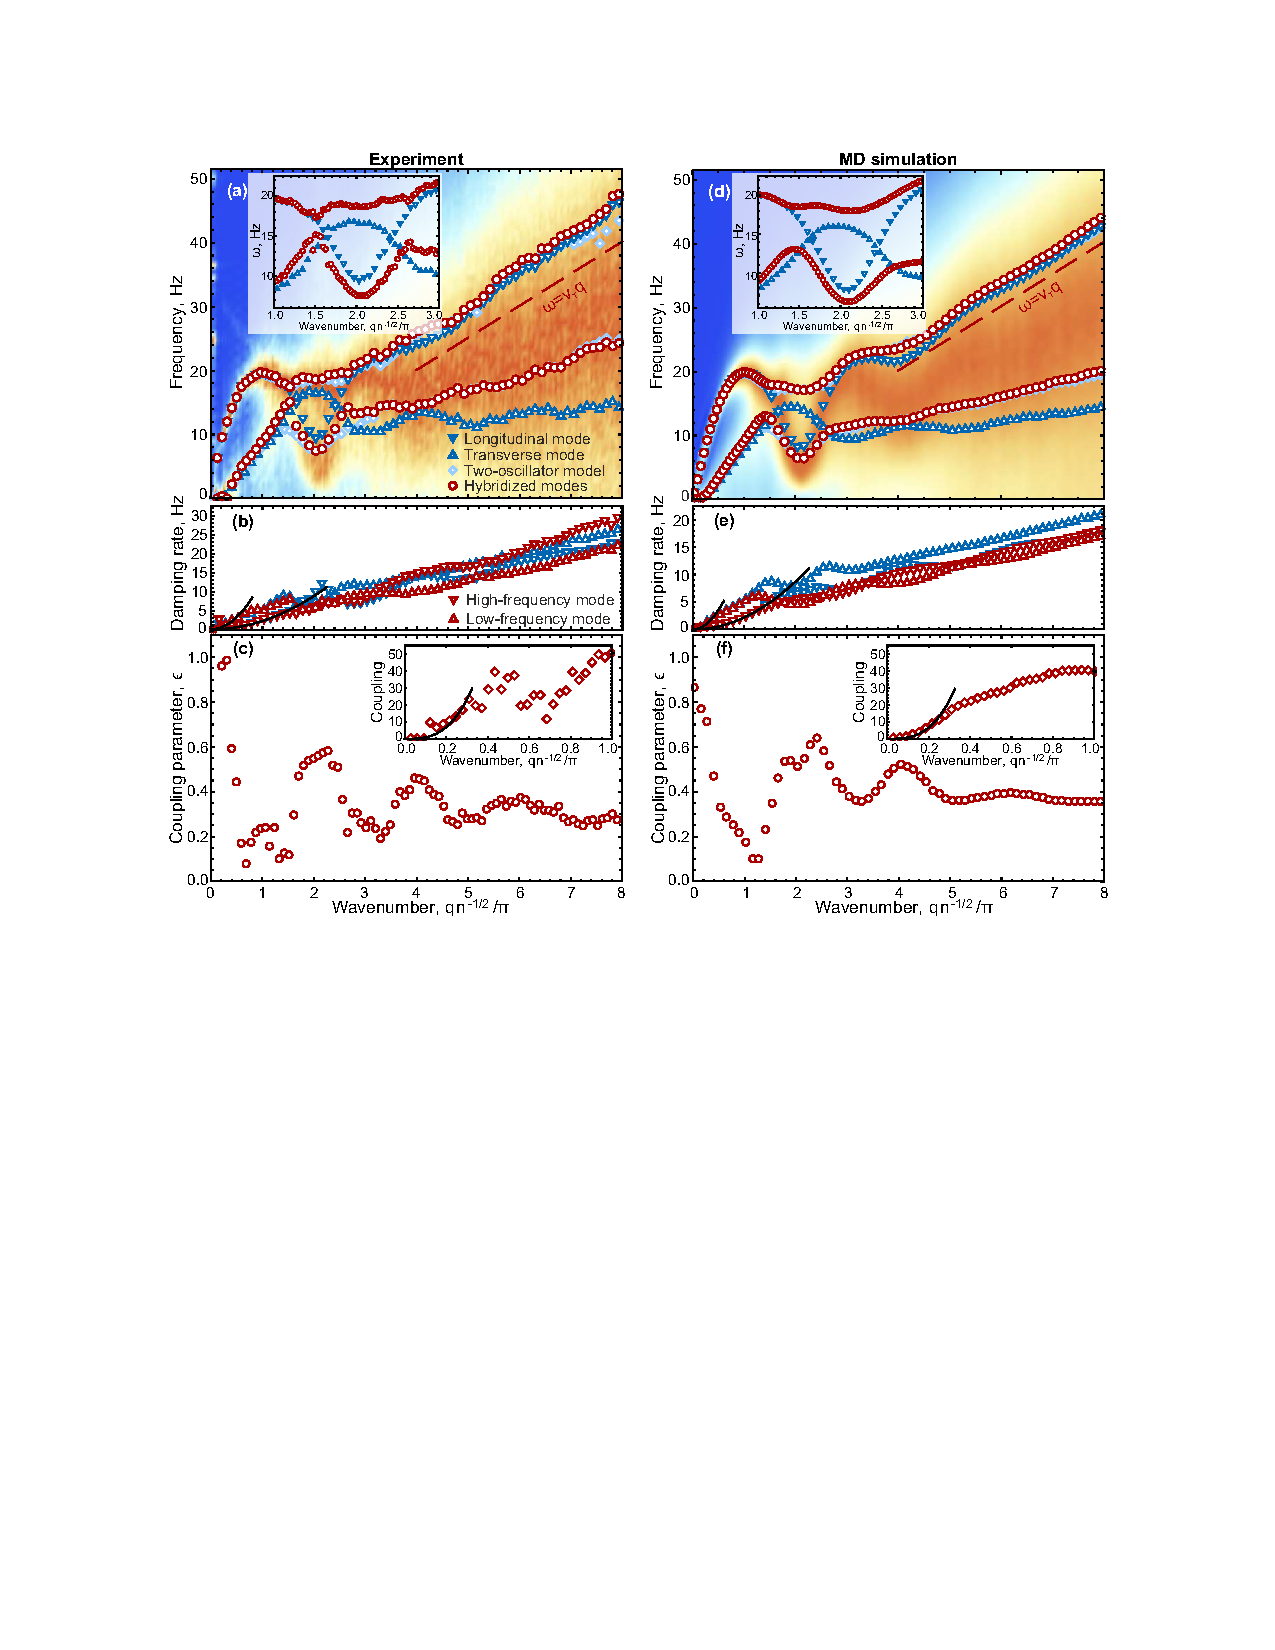
\includegraphics[width=0.7\textwidth]{Ris/Plasma_SP_3.pdf}
    \caption{Амплитуды и спектры возбуждений для квазидвумерной жидкости с потенциалом Юкавы. }
    \label{PlasmaSp}
    \end{center}
\end{figure}

На (a) - (c) изображены спектры, скорости затухания и параметры связи между продольными и поперечными возбуждениями, полученные в ходе эксперимента, а на панелях (d) - (f) - результаты, полученные методом МД.

Видно, что данные, полученные в ходе эксперимента, согласуются с результатами МД. Наблюдаемые различия обусловлены лучшей статистикой МД и более сложными взаимодействиями в эксперименте из-за плазменных вейков. Антикроссинг мод наблюдается при $q^{-1/2} \pi^{-1} \approx 1.6$ или $2.4$ (в диапазоне волновых чисел между коллективной и одночастичной динамикой), где две пересекающиеся моды (показанные синими треугольниками) отталкиваются друг от друга. В результате антикроссинга наблюдается высокочастотные и низкочастотные моды гибридизированных возбуждений, представленные красными кругами на рис.  \ref{PlasmaSp}(a) и  \ref{PlasmaSp}(d) вместо продольных и поперечных возбуждений, показанных синими треугольниками.

\begin{figure}[htbp]
\begin{center}
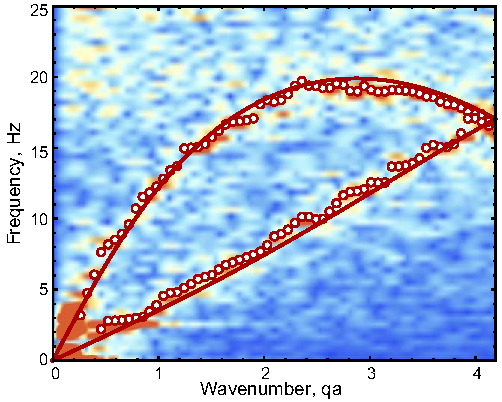
\includegraphics[width=0.6\textwidth]{Ris/Plasma_SP_1.pdf}
\caption{Спектры возбуждений для кристалла с потенциалом Юкавы.}
\label{PlasmaSp2}
\end{center}
\end{figure}

В жидкостях возбуждения сильно демпфированы и поэтому продольная и поперечная составляющие амплитуды $C(q, \omega) = C_{\parallel}(q, \omega) + C_{\perp}(q, \omega)$, показанные на рис.  \ref{PlasmaSp}(a) и  \ref{PlasmaSp}(d) оказываются размытыми в плоскости $(q,\omega)$.  Скорости затухания представлены на рис.  \ref{PlasmaSp}(b) и \ref{PlasmaSp}(e). Сплошные черные линии показывают для эксперимента и моделирования диффузионное затухание $\Gamma_{\parallel, \perp} \sim q^2$ на небольших $q$. Безразмерный параметр связи $\varepsilon$ показан на рис.  \ref{PlasmaSp}(c) и \ref{PlasmaSp}(f) для эксперимента и моделирования МД. Сплошная черная линия на (c), (f) -  это результаты аппроксимации $\varepsilon \Omega_{\parallel, \perp} \sim q^3$. Данное соотношение получается из того, что при малых $q$ $ \Omega_{\parallel} \approx   \omega_{\perp} \sim q$, а $\Omega_{\perp} \approx   \omega_{\parallel} \sim q^2$.



Фононный спектр в комплексной (пылевой) плазме изображен на рис. \ref{PlasmaSp2}: амплитуды показаны в цветовом формате; красные символы показывают дисперсионные соотношения $\omega_{\parallel, \perp}(q)$ для продольных и поперечных колебаний, полученные путем аппроксимации экспериментально полученных значений $C(q, \omega)$ моделью затухающего гармонического осциллятора. Сплошная красная линия соответствует теоретическим дисперсионным соотношениям для кристаллов с потенциалом Юкавы.


\section{Выводы}

Метод, основанный на модели 2DHO, пригоден для анализа возбуждений в
 в двумерных и трехмерных жидкостях с различными потенциалами взаимодействия. Однако в длинноволновом пределе наблюдается возврат к режиму индивидуальной динамики частиц, при котором
продольные и поперечные спектры потока определяются распределениями Максвелла по скоростям.

Полученные результаты могут быть применены для анализа возбуждений в жидкой комплексной (пылевой) плазме.
Так же с помощью данного подхода можно детального анализировать возбуждения в жидких средах различной природы, от
простых жидкостей и благородных газов до жидких металлов, молекулярных и сложных жидкостей. Смешивание мод в сильно связанных жидкостях приводит к эффективному взаимодействию между продольными и поперечными возбуждениями, что приводит к антикроссингу мод. Детальный анализ возбуждений открывает захватывающие перспективы для установления  соотношений между индивидуальной, коллективной динамиками и
термодинамикой жидкостей. 
